%%%%%%%%%%%%%%%%%%%%%%%%%%%%%%%%%%%%%%%%%%%%%%%%%%%%%%%%%%%%%%%%%%%%%%%%%%%%%%%%
\section{Interpretação corporal da música}
\label{sec:interpretacioncorporal}

\begin{comment}
\begin{figure}[t]
\begin{elaboracion}{Que é o ``flow''?}
\label{page:flow}
\index{Musicalidade!Flow}
\textcolor{red}{Nós nos perdemos no movimento e na música,
esquecendo as restrições do tempo e da normalidade, este fenomeno é conhecido como ``Flow''} \cite{czikszentmihalyi1990flow} \cite{trehub2003developmental}.
\end{elaboracion}
\label{fig:flow}
\end{figure}
\end{comment}

Seguindo as Definições \ref{def:MusicalidadeNaDanca} e \ref{def:MusicalidadeNaDancaIT},
para que um dançarino tenha musicalidade, este precisa primeiro interiorizar as informações que traz a música,  
esse processo é chamado de \hyperref[cap:percepcaomusical]{\textbf{percepção musical}} 
e foi abordado no Capítulo \ref{cap:percepcaomusical}.
Uma vez percebida e desfragmentada a música em aspectos mediante a percepção musical,
o dançarino escolhe os que considera mais interessantes para serem incluídos na sua dança.
Com esse fim faz um mapeamento desses aspectos musicais a aspectos mecânicos ou ideias de movimentos (aspectos do movimento).
Essas ideias, que são nosso projeto de dança, logo serão trazidas à realidade mediante nossa interpretação corporal, 
que não é um processo livre de erros, o qual estará influenciado por fatores externos (entorno de dança) e 
internos (capacidade de realização).
Todo o processo de interpretação da música pode ser visto de forma diagramática na Figura \ref{fig:interpretacion-corporal}.
\begin{figure}[!h]
  \centering
    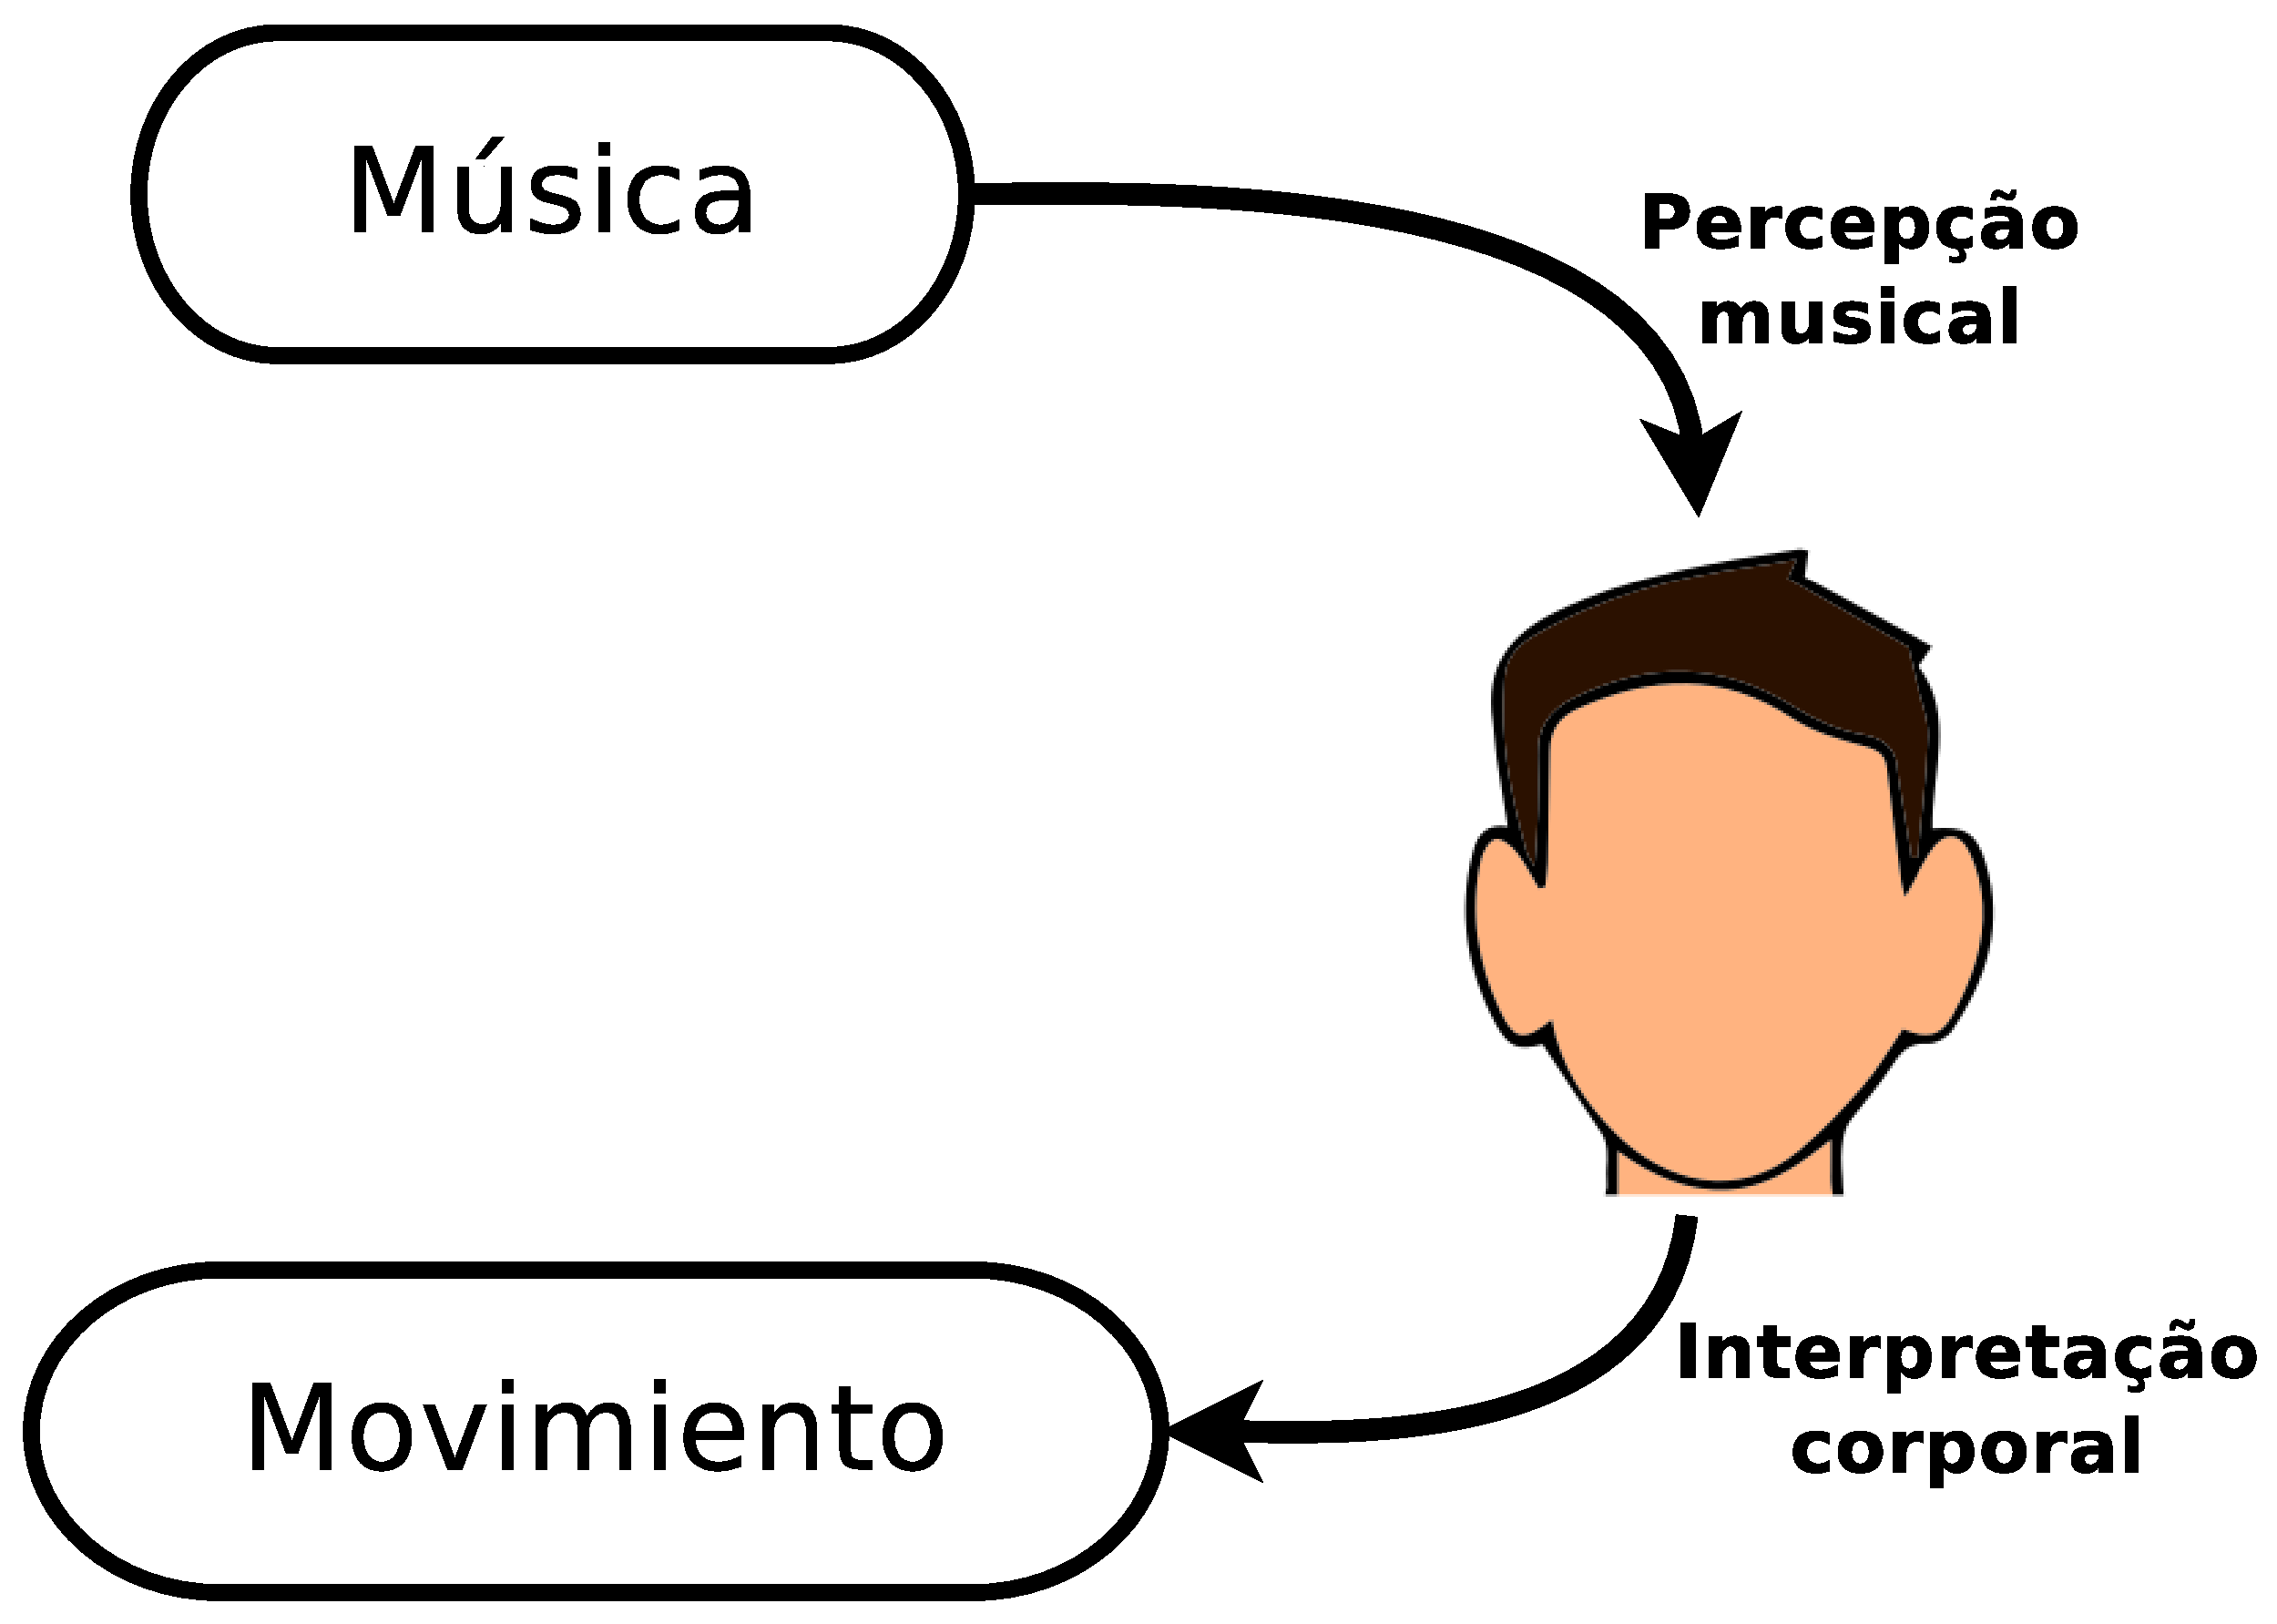
\includegraphics[width=1.00\textwidth]{chapters/cap-musicalidade/interpretacion-corporal.eps}
\caption{Interpretação corporal da música.}
\label{fig:interpretacion-corporal}
\end{figure}

O mapeamento entre aspectos da música e aspectos do movimento 
pode ser feito de forma direta ou de forma simbólica, como é mostrado na Figura \ref{fig:mapeamento};
por exemplo:
\begin{itemize}
\item Um aspecto da música, como um motivo melódico,
pode ser mapeado diretamente extraindo o ritmo e vinculando-o a um movimento de pés (ex: intenção de fazer um Romário, um pulo, etc.);
\item ou este motivo pode ser primeiro interpretado como um sujeito, situação ou ideia simbólica,
como o amor, para logo esta ideia ser atrelada\footnote{O 
processo de atrelamento simbólico da música é conhecido como \hyperref[sec:leitmotivdanca]{\textbf{leitmotiv}}, 
e é estudada no âmbito da dança na Seção \ref{sec:leitmotivdanca}.} a um aspecto do movimento, como um abraço.  
\end{itemize}

\begin{figure}[!h]
  \centering
    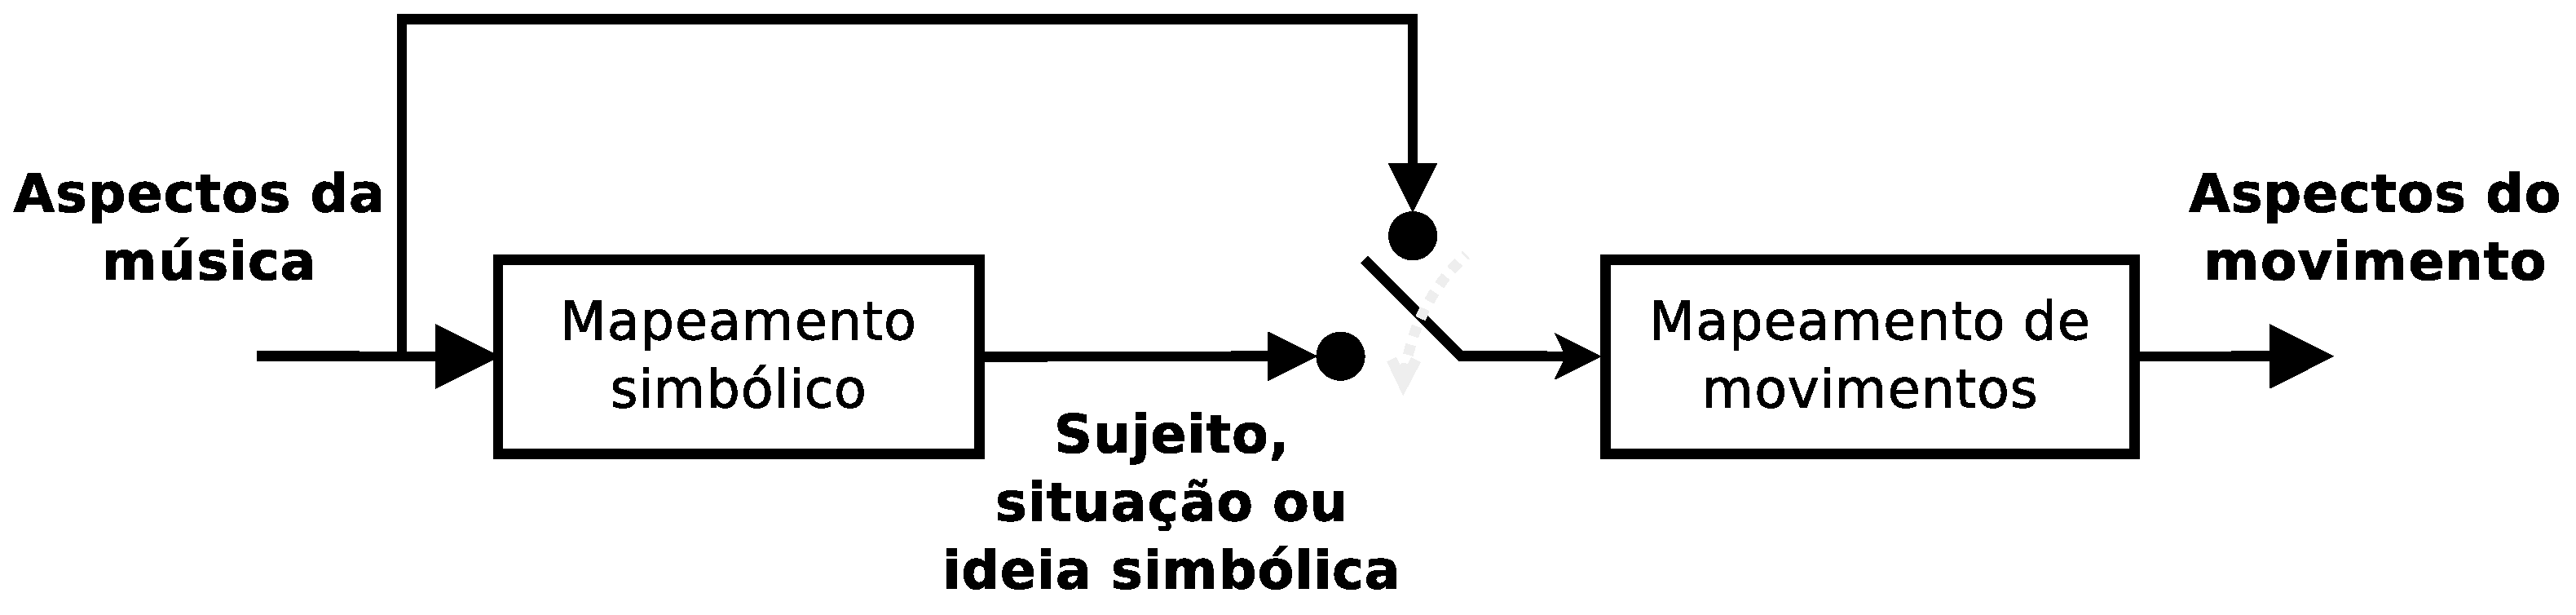
\includegraphics[width=1.00\textwidth]{chapters/cap-musicalidade/mapeamento.eps}
\caption{Mapeamento de ideias e estimulos a movimentos.}
\label{fig:mapeamento}
\end{figure}


As formas em que um dançarino interpreta a informação musical estão amplamente estudadas, 
não só no âmbito da dança se não que de forma geral no âmbito das artes cênicas;
entre os pontos de estudo mais difundidos 
para a interpretação de ideias mediante o uso do corpo, podemos encontrar:
\begin{itemize}
\item A \hyperref[sec:BodyAwareness]{\textbf{consciência corporal}},
\item o \hyperref[sec:BodyControl]{\textbf{controle corporal}},
\item a \hyperref[sec:BodyIsolation]{\textbf{dissociação corporal}}, e
\item a \hyperref[sec:BodyExpression]{\textbf{expressão corporal}}.
\end{itemize}
Para conhecer as definições e mais detalhes de como podemos aprimorar estes tópicos,
invito aos leitores a ir ao Capítulo \ref{fig:bodyrelations}.

No caso da dança a dois, o dançarino usa todos estes elementos 
para enviar ou projetar corporalmente uma informação que tenha coerência (informação mutua) com a música que percebe.
Os receptores ou destinatários destas informações podem ser: o par de dança,
o público, ou o próprio dançarino; 
assim, dependendo do âmbito em que este se desenvolva,
podem incluso ser todos eles ao mesmo tempo os receptores da informação.

O dançarino tem muita liberdade criativa quando realiza o 
mapeamento entre os aspectos da música e do movimento, 
pois neste ponto podem ser introduzidas subjetividades. 
Por exemplo imaginemos que, metaforicamente, um aspecto da música recopilado pelo dançarino 
está representado pela Figura \ref{fig:LaCopaDeRubin}.
Nesse caso, uma pergunta interessante seria se 
o dançarino fará um mapeamento para um movimento de bêbados (um copo de vinho) ou de namorados (duas caras)?
\begin{figure}[!h]
  \centering
    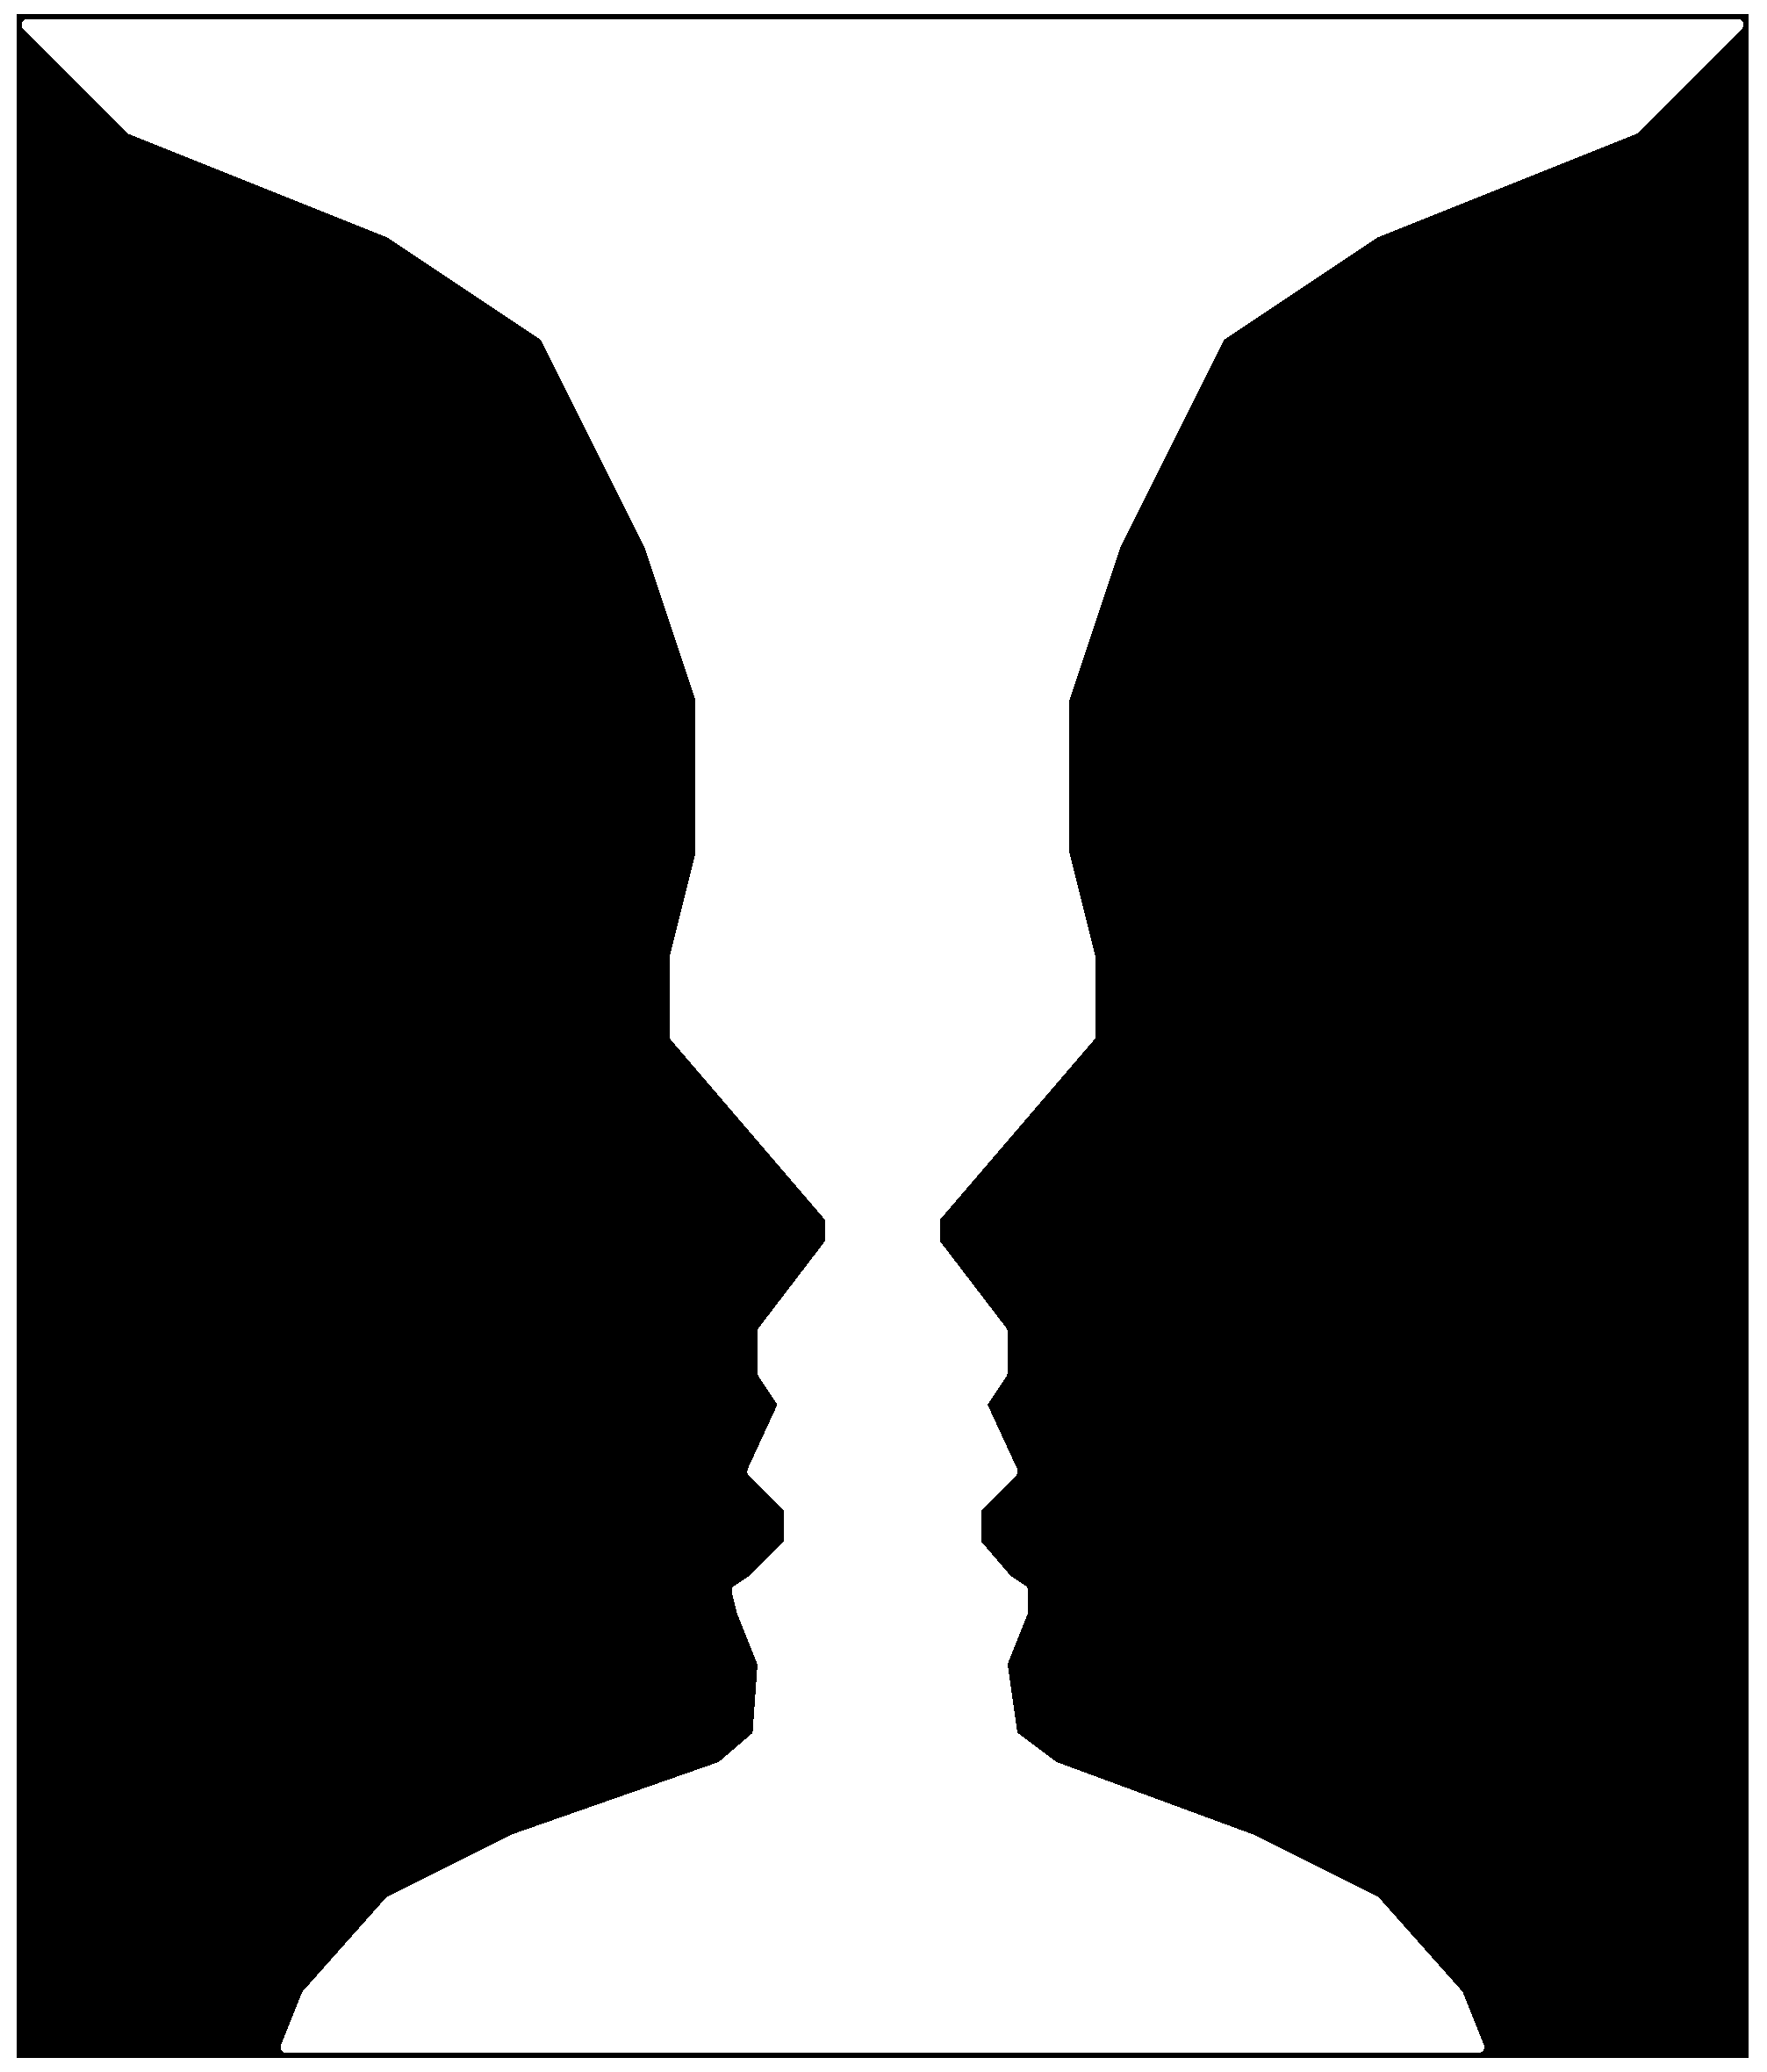
\includegraphics[width=0.43\textwidth]{chapters/cap-musicalidade/LaCopaDeRubin.eps}
\caption{A perspetiva do interprete.}
\label{fig:LaCopaDeRubin}
\end{figure}

O objetivo dos próximos  capítulos não é primariamente indicar ao leitor se na Figura \ref{fig:LaCopaDeRubin} 
existe um copo ou duas pessoas se olhando frente a frente, e sim desenvolver técnicas ou 
apresentar treinamentos para ajudar-nos a projetar qualquer destas duas perspetivas, 
seguindo a interpretação de cada dançarino.

\begin{FraseFernandoPR}{Escolhas}
Muitas vezes você notará que não existe um caminho correto 
e sim motivos corretos para escolher um caminho.%%23/07/2013
\end{FraseFernandoPR}

\begin{figure}[!h]
\begin{elaboracion}{Nossos problemas com a musicalidade}
\index{Música!Teste}
Um auto exame interessante a ser feito por nós, é analisar a Figura \ref{fig:interpretacion-corporal},
e observar em que parte de  nosso processo para aumentar nossa musicalidade  
(que inicia na música e termina em nosso movimento) estamos tendo problemas. Por exemplo:
\begin{itemize}
\item Se temos problemas em obter os aspectos da música, 
então temos problemas com nossa percepção musical,
e devemos procurar treinamentos e informação relativa a esse tema;
alguns pontos sobre o assunto estão disponíveis no Capítulo \ref{cap:percepcaomusical}.
\item Se já dividimos a música em aspectos, e não sabemos que ação ou movimento lhe corresponde,
então temos um problema no mapeamento dos aspectos;
este tema é muito subjetivo e depende da perspetiva de cada um;
porém existem algumas técnicas e recomendações que são comumente usadas,
como as descritas nas Seções \ref{sec:mikeymousing}, \ref{sec:leitmotivdanca}, 
\ref{sec:seguindoinstrumentos} e \ref{sec:musicalidadetensionrelease}.
\item Se já temos  ideia dos movimentos que faremos em cada aspecto escolhido da música,
mas temos problemas em levar estes movimentos desde o mundo da imaginação à realidade;
então temos um problema com nossa interpretação corporal;
algumas informações relativas a este assunto podem ser vistas no Capítulo  \ref{fig:bodyrelations}.
\end{itemize}
\end{elaboracion}
\label{fig:testemusicalidade}
\end{figure}

